\documentclass[10pt,a5paper]{article} 
\renewcommand{\baselinestretch}{1.0}
\usepackage{cite}
\usepackage[dvips]{graphicx}
\usepackage{psfrag}
\usepackage{color}
\usepackage[cmex10]{amsmath}
\usepackage{amsfonts} 
\usepackage[font=footnotesize, captionskip=10pt]{subfig}
\usepackage{tikz}
\usepackage{flushend}
\usepackage{times}
\usepackage[margin=1.5cm]{geometry}

\usepackage[slovak]{babel}
\usepackage[utf8]{inputenc}
\usepackage[T1]{fontenc}

\pagestyle{empty}

\hyphenation{net-works}
\newtheorem{remark}{Remark}

\begin{document}

\title{Paper title}
\author{Michal Chovanec\\
michal.chovanec@yandex.com}
\date{}
\maketitle 
\thispagestyle{empty}

%\noindent$^1$\ affiliation\\
%\noindent$^2$\ affiliation\\

\noindent {\bf Keywords:} keywords...

\noindent {\bf Abstract:} Abstract

\section{Introduction}

Úvod ~\cite{bib:Aproximation}.
ľ š ť ž  \\
č ý á í é ú ä ô ň \\

\begin{equation}
\label{McCulloch_Pitts}
  y(n) = \varphi(\sum_{i = 0}^{N-1} x_i(n)w_i(n))
\end{equation}


\section{Dalsia cast}

\begin{figure}[!ht]
\centering
%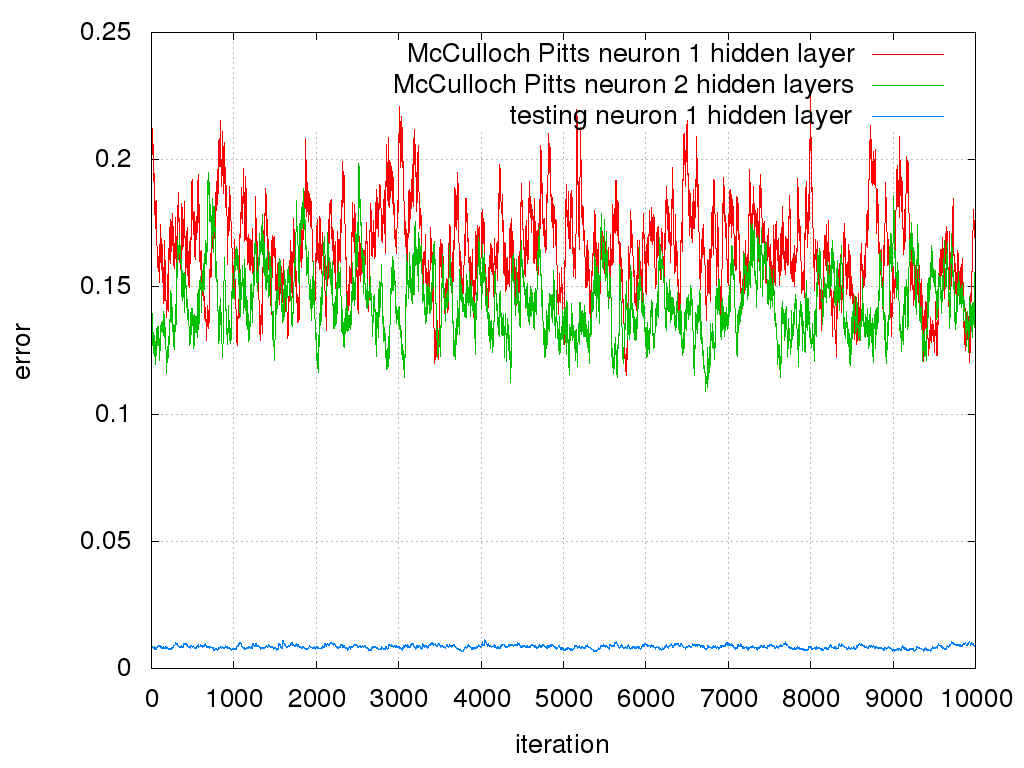
\includegraphics[width=2.5in]{multiplexer_result.png}
\caption{Obrazok}
\label{obrazok}
\end{figure}

\section{Zaver}


\bibliographystyle{IEEEtran}
\bibliography{bib}

\begin{thebibliography}{4}

\bibitem{bib:Aproximation} Kolmogorov's Theorem,
http://neuron.eng.wayne.edu/tarek/MITbook/chap2/2\_3.html


\end{thebibliography}



\end{document}
